\begin{figure}[htbp]
\centering
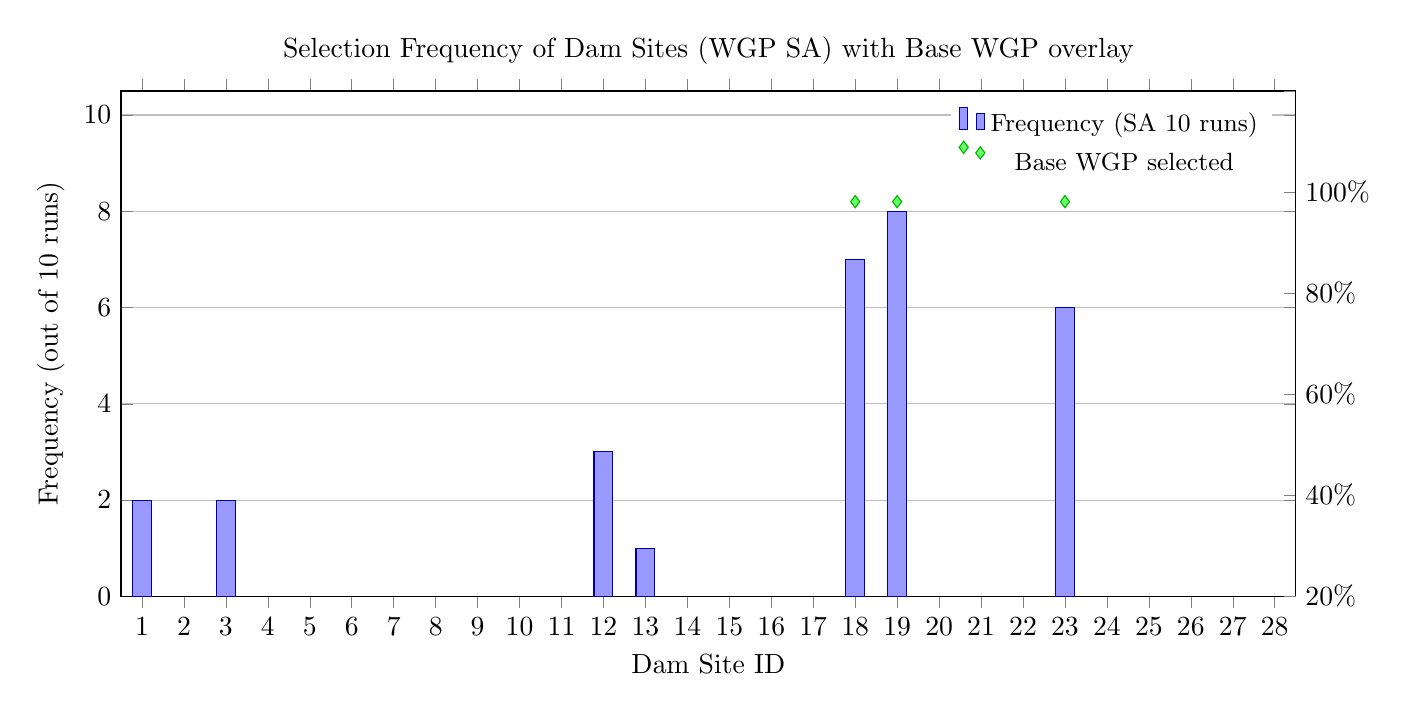
\begin{tikzpicture}

% =======================
% Left axis: Frequency bars (0..10)
% =======================
\begin{axis}[
  title={Selection Frequency of Dam Sites (WGP SA) with Base WGP overlay},
  xlabel={Dam Site ID},
  ylabel={Frequency (out of 10 runs)},
  ymin=0, ymax=10.5,
  xmin=0.5, xmax=28.5,
  xtick={1,2,...,28},
  width=16.5cm, height=8cm,
  ymajorgrids,
  bar width=0.45,
  ybar,
  legend style={font=\small, at={(0.98,0.98)}, anchor=north east, draw=none, fill=white},
]

% --- Frequency bars (hard-coded; 10 SA runs) ---
% Non-zero frequencies:
\addplot+[fill=blue!40!white, draw=blue!70!black] coordinates {
  (1,2) (3,2) (12,3) (13,1) (18,7) (19,8) (23,6)
};
\addlegendentry{Frequency (SA 10 runs)};

% --- Base WGP selections as red diamonds (placed slightly above max) ---
\addplot+[only marks, mark=diamond*, mark size=2.2pt, draw=green!70!black, fill=green!60] coordinates {
  (18,8.2) (19,8.2) (23,8.2)
};
\addlegendentry{Base WGP selected};

\end{axis}

% =======================
% Right axis: Percent labels (0..100%)
% =======================
\begin{axis}[
  hide x axis,
  axis y line*=right,
  ymin=0, ymax=10.5,
  ytick={0,2,4,6,8,10},
  yticklabels={0\%,20\%,40\%,60\%,80\%,100\%},
  width=16.5cm, height=8cm,
]
\end{axis}

\end{tikzpicture}
\caption{Summary of dam-site selection frequency across 10 WGP sensitivity runs; red diamonds mark sites selected by the Base WGP solution. Right axis shows percent of runs.}
\label{fig:wgp_sa_frequency}
\end{figure}
        